\chapter{One Dimensional Advection}
\section{Introduction}
Advection is one of the most fundamental phenomena in meteorology as it describes the
transport of aerosols, fluids, and humidity. The simplest case can be described by the
linear advection equation
\begin{align}
    \label{eq:adv}
    \frac{\partial u}{\partial t} + c \frac{\partial u}{\partial t} = 0
\end{align}
for a constant $c\in\mathbb R$ and a function $u: I \times \mathbb R_{\geq 0} \to 
\mathbb{R}$ with the interval $I \subset \mathbb R$. In many applications, the constant 
$c$ models the direction and velocity of the transported substance. 
Equation \eqref{eq:adv} is a
building block to more complicated equations like the diffusion-advection equation, Burger's
equation, or the Navier-Stokes equation but is more tractable than the higher order or
nonlinear equations.

We consider the advection equation~\eqref{eq:adv} with $I = [a,b]$ and periodic boundary
conditions, i.e. $u(a) = u(b)$ and the initial values $u(x,0) = u_0(x)$ with $u_0(t): I \to \mathbb R$. W.l.o.g.
we can assume $a = 0$ and a solution is given by
\begin{align}
    u(x,t) = u_0(x - ct)
\end{align}
with $u_0$ for the initial values and the minus is implicitly taken $\mod b$, see
\cite{Evans2010} for details. 

Since we have an explicit solution, we can use it as a 
benchmark problem for testing different
numerical methods. In this work we test the donor cell scheme, the leap frog scheme,
the Lax-Wendroff scheme, van Leer scheme, and the method of lines with a 4th order
Runge Kutta time integrator. 

In this work, we test these numerical methods on the test problem in equation~\eqref{eq:adv}
with $I = [0, 100]$ and the initial values
\begin{align}
    \label{eq:init}
    u_0(x) = \begin{cases}
        1 & x \in (5,15) \\
        0 & \text{otherwise}
    \end{cases}.
\end{align}
The solution of \eqref{eq:adv} with the initial values~\eqref{eq:init} is a shock solution 
as it exhibits discontinuities.

In section 2 we present the numerical methods used in the evaluation and their properties. Furthermore, we present the evaluation metrics and their significance for numerical
meteorology.
In the following section 3, we present the results of our investigation and conclude with section 4.

\section{Methods}

We consider the linear advection equation defined in~\eqref{eq:adv} on the
interval $(1, 100)$ with the spatial discretization of $\Delta x= 1.0$ and time step size
$\Delta t = 1.0$ and the advection speed $c = 0.5$. Then the Courant-Friedrichs-Lewy number
is given by
\begin{align*}
    \mathrm{CFL} = \frac{c \Delta t}{\Delta x} = 0.5
\end{align*}
and thus conditional stable schemes are stable. We use the initial condition as 
in~\eqref{eq:init} for testing the numerical schemes, which we introduce in the following.

\subsection{Donor Cell Method}
The Donor Cell Method (also called the upwind scheme) is the simplest finite-difference
method for solving the linear advection equation~\eqref{eq:adv}. Its stability criterion
was first analyzed by Courant, Friedrichs, and Lewy \cite{Courant1928}, and a modern
presentation can be found in LeVeque’s text \cite{LeVeque2002}. The key idea is to use
the characteristic flow direction to choose the finite-difference stencil: for $c>0$
one uses a backward (upwind) difference, whereas for $c<0$ one uses a forward
(upwind) difference. By using an Euler Step in time we arrive at:
\begin{align*}
    u^{n+1}_j = u^n_j + \frac{c \Delta x}{\Delta t}(u^n_{j} - u^n_{j-1})
\end{align*}
for positive $c$. With $u^n_{j}$ we denote the discrete solution of equation~\eqref{eq:adv},
with $n$ as the time index and $j$ as the spatial index. This scheme uses first-order
finite difference quotients in space and time, so we have an order of convergence of $\Delta x$.

\subsection{Leap Frog Method}
The Leap Frog Method is a finite difference method, with second order accuracy in space and
time \cite{Durran2010}. This leads to:
\begin{align*}
    \frac{u_j^{n+1} -u_j^{n-1}}{2\Delta t} = c \frac{u^n_{j+1} - u^n_{j-1}}{2\Delta x} = 0
\end{align*}
If the absolute $\mathrm{CFL}$-number is smaller than one, then this scheme is stable.
Since we need two steps, we compute the first step with an Euler Step, i.e. we use a first
foward difference of first-order to approximate the values of $u^2_j$.
\subsection{Lax-Wendroff Method}
The Lax-Wendroff Method is a finite volume method which is based on the Divergence
Theorem. The hyperbolic equation is written as an integral equation over a control
volume, i.e.
\begin{align*}
    \frac{\partial u}{\partial t} + \operatorname{div} f(u) = 0
\end{align*}
implies that for a control volume, like a cell $V$, we have
\begin{align*}
    0 &= \int_V\frac{\partial u}{\partial t} + \operatorname{div} f(u) \; dx \\
    &= |V| \frac{\partial \bar u_V}{\partial t} + \int_V \operatorname{div} f(u) \; dx \\
    &= |V| \frac{\partial \bar u_V}{\partial t} + \int_{\partial V} f(u) \cdot \nu \; dS.
\end{align*}
Here $\bar u_V$ is the average over the control volume $V$ and in the second step
we used the Divergence Theorem. Finite Volume methods discretize the flux through the
boundary of the control volume, which is in practical implementation a cell. This leads
to the master equation for one dimensional problems, as:
\begin{align}
    \label{eq:fvm}
    \frac{u^{n+1}_j - u^n_j}{\Delta t} + \left( \frac{F_{j + \tfrac{1}{2}} - F_{j - \tfrac{1}{2}}}{\Delta x}\right) = 0
\end{align}
with $F_{j \pm  \tfrac{1}{2}}$ as the approximated flux through the right,
respectively left, boundary of the one-dimensional cell. 

The Lax-Wendroff scheme is given by the flux:
\begin{align*}
    F_{j -\tfrac{1}{2}}^n = \frac{1}{2}c (u_{j-1}^n + u^n_j) - \frac{1}{2}\frac{\Delta t}{\Delta x}c^2(u^n_j - u^n_{j-1})
\end{align*}
which is a second-order approximation\cite{LeVeque2002}.

\subsection{Van Leer Method}
The Van Leer Method is another finite volume method which combines a higher order flux 
approximation with a lower order one using a flux limiter function, i.e.
\begin{align*}
    F_{j - \tfrac{1}{2}} = F_{j - \tfrac{1}{2}}^{\mathrm{low}} + \phi(r)\left( F_{j - \tfrac{1}{2}}^{\mathrm{high}}  - F_{j - \tfrac{1}{2}}^{\mathrm{low}} \right)
\end{align*}
where $F_{j - \tfrac{1}{2}}^{\mathrm{low}}$ is the low order flux and 
$F_{j - \tfrac{1}{2}}^{\mathrm{high}} $ the high order flux. The parameter $r$ is the
ratio of differences of the cell values in the upwind direction. The idea behind the
flux limiter is to detect shocks and switch to an appropriate approximate flux.
The function $\phi(r)$ is the flux limiter function and throughout literature,
different functions are proposed, see \cite{LeVeque2002} for commonly used ones. The Van 
Leer method uses as a flux limiter the following function as proposed in \cite{Leer1979}:
\begin{align*}
    \phi(r) = \frac{r + |r|}{1 +  |r|}.
\end{align*}
As a lower-order flux we use the flux from the donor cell method, i.e.
\begin{align*}
    F_{j - \tfrac{1}{2}}^{\mathrm{low}} = c u_J
\end{align*}
where $J$ is the index in the upwind direction.

\subsection{Method of Lines}
The idea behind the Method of Lines is to discretize the spatial variable and its 
derivatives and consider it as the right hand side of an ordinary differential 
equation (ODE) and use an ODE solver to approximate the solution. Formally this means
\begin{align*}
    \frac{\partial u}{\partial t} = D_x u \approx \hat D_x u
\end{align*}
where $\hat D_x u$ is an approximation of the differential operator $D_x$ with respect
to the spatial variable $x$. We use the classical fourth-order explicit Runge-Kutta
method to approximate the time derivative and use a fourth-order finite difference stencil
in space, i.e.
\begin{align*}
    \frac{\partial u}{\partial t}\vert_{u = u_i} = \frac{1}{h}\frac{u_{i-2} - 8u_{i-1} + 8u_{i+1} - u_{i+2}}{12},
\end{align*}
with the discretization parameter $h > 0$.


\subsection{Implementation}
We implement each method in the programming language \texttt{Julia} by constructing
sparse matrices which represent finite difference operators for the finite difference schemes. The
finite volume methods compute directly the flux to the solution and then apply it to 
equation~\eqref{eq:fvm}. We use the packages \texttt{Plots} and \texttt{PrettyTables} for 
postprocessing our simulation data. The code is available under \url{https://github.com/NiclRich/NumericalMeteorology}.

The code documentation was created with the help of ChatGPT version 5; however, we refrained from
code generation as the generated code we tested yields unreliable results and not efficient code.
Our implementation heavily relies on vectorization of the quantities for applying faster routines
and ChatGPT often gives inefficient code\footnote{For the details of vectorization see also
\cite{Bezanson2017}. However, the code does work in principle as it can be seen in this blog
post from the Julia community: \url{https://www.stochasticlifestyle.com/chatgpt-performs-better-on-julia-than-python-and-r-for-large-language-model-llm-code-generation-why/}}.

\section{Results}
We evaluate the methods using the following diagnostics. By $\tilde{u}_i^n$, we denote the numerical
solution.
\begin{enumerate}
    \item \emph{RMSE}: The root mean square error is given by:
    \begin{align*}
        \mathrm{RMSE}^n = \sqrt{\frac{1}{M}\sum_{i=1}^M (u_i - \tilde u_i)^2}
    \end{align*}
    which approximates the $L^2$-distance between the numerical solution and the
    exact solution.

    \item \emph{RM}: The mass ratio measures the conservation properties of the scheme. Hyperbolic
    equations often arise from conservation principles like the conservation of mass or momentum. 
    It compares the initial mass\footnote{This is a generic name for the conserved quantity. For
    different equations, the term mass can refer to different quantities.} to the mass at the
    next time steps and it is defined as:
    \begin{align*}
        \mathrm{RM}^n = \frac{\sum_{i=1}^M u_i^n}{\sum_{i=1}^M u_i^0}.
    \end{align*}

    \item \emph{RMP}: The mass ratio has the disadvantage that it does not capture undershoots which can
    balance the mass ratio. Thus the positive mass ratio is introduced to measure only the positive mass
    which is physically more important. It is defined as
    \begin{align*}
        \mathrm{RMP}^n = \frac{\sum_{i=1}^M \max(u_i^n, 0)}{\sum_{i=1}^M \max(u_i^0, 0)}.
    \end{align*}

    \item \emph{MDR}: Some conservation equations also conserve the higher order integrals, like the
    Korteveg-de-Vries equation. The measure the energy preserving properties of the scheme, as some
    schemes preserves them and some are dissipating. An increasing energy is a sign for 
    instability. In many situations the $L^2$-norm is conserved which is often denoted as energy. The
    discrete energy ratio is defined as:
    
    \begin{align*}
        \mathrm{MDR}^n =\frac{\sum_{i=1}^M (u_i^n)^2}{\sum_{i=1}^M (u_i^0)^2}.
    \end{align*}

    \item \emph{RMAX} and \emph{RMIN}: Some schemes show overshoots and undershoots,
    i.e. we observe higher
    or smaller values while advancing time steps, which is not physical. To 
    measure this effect, we consider
    the ratio of the minimum / maximum at the time comparing the minimum and maximum
    to the range of observed 
    initial values, it is defined as:
    \begin{align*}
        \mathrm{RMAX}^n = \frac{\max_i u_i^n}{\max_i u_i^0 - \min u_i^0}, \\[1em]
        \mathrm{RMIN}^n = \frac{\min_i u_i^n}{\max_i u_i^0 - \min u_i^0}. \\
    \end{align*}    
\end{enumerate}
We see that each method captures different effects of the solution. The results of the diagnostics can be found in table~\ref{tab:diag}.

\begin{table}[ht]
    \centering
    \resizebox{\textwidth}{!}{%
    \begin{tabular}{rrrrrrrr}
  \hline
  \textbf{Method} & \textbf{time step} & \textbf{RMSE} & \textbf{RM} & \textbf{RMP} & \textbf{MDR} & \textbf{RMAX} & \textbf{RMIN} \\\hline
  Donor Cell & 1 & 0.0 & 1.0 & 10.0 & 10.0 & 1.0 & 0.0 \\
   & 5 & 0.0640588 & 1.0 & 10.0 & 8.90625 & 1.0 & 0.0 \\
   & 10 & 0.0894259 & 1.0 & 10.0 & 8.33076 & 1.0 & 0.0 \\
   & 90 & 0.158055 & 1.0 & 10.0 & 5.0725 & 0.710904 & 0.0 \\
   & 180 & 0.13913 & 0.527255 & 5.27255 & 2.08121 & 0.545105 & 0.0 \\
  Leap Frog & 1 & 0.0 & 1.0 & 10.0 & 10.0 & 1.0 & 0.0 \\
   & 5 & 0.0926835 & 1.00031 & 10.5391 & 10.0109 & 1.30428 & -0.304275 \\
   & 10 & 0.110387 & 1.04498 & 11.0802 & 9.93826 & 1.25791 & -0.25689 \\
   & 90 & 0.240319 & 1.49998 & 18.1111 & 12.5363 & 1.12702 & -0.513902 \\
   & 180 & 0.787427 & 2.62771 & 31.7361 & 70.677 & 4.48806 & -1.71463 \\
  Lax Wendroff & 1 & 0.0 & 1.0 & 10.0 & 10.0 & 1.0 & 0.0 \\
   & 5 & 0.0630742 & 1.0 & 10.2205 & 9.60284 & 1.11401 & -0.114014 \\
   & 10 & 0.0871998 & 1.0 & 10.2827 & 9.46365 & 1.15495 & -0.154948 \\
   & 90 & 0.11688 & 1.0 & 10.7514 & 8.94465 & 1.17196 & -0.20807 \\
   & 180 & 0.18301 & 1.0 & 10.9953 & 8.74376 & 1.11346 & -0.176601 \\
  van Leer & 1 & 0.0 & 1.0 & 10.0 & 10.0 & 1.0 & 0.0 \\
   & 5 & 0.0616396 & 1.0 & 10.0 & 8.95601 & 1.0 & 0.0 \\
   & 10 & 0.0835335 & 1.0 & 10.0 & 8.4976 & 1.00003 & 0.0 \\
   & 90 & 0.134863 & 1.0 & 10.0 & 5.93146 & 0.817658 & 1.61559e-27 \\
   & 180 & 0.182107 & 1.0 & 10.0 & 4.77261 & 0.665345 & 1.36306e-13 \\
  RK4 & 1 & 0.0 & 1.0 & 10.0 & 10.0 & 1.0 & 0.0 \\
   & 5 & 0.0781667 & 1.0 & 10.568 & 9.99845 & 1.21119 & -0.211342 \\
   & 10 & 0.091589 & 1.0 & 10.8883 & 9.99653 & 1.22599 & -0.322765 \\
   & 90 & 0.125852 & 1.0 & 12.7034 & 9.96686 & 1.2117 & -0.289821 \\
   & 180 & 0.24135 & 1.0 & 13.1665 & 9.93589 & 1.22085 & -0.343274 \\\hline
\end{tabular}

    }
    \caption{Numerical Diagnostics for the solution of the linear advection equation.}
    \label{tab:diag}
\end{table}
The donor cell scheme yields a RMSE comparable with the other methods except the van Leer scheme,
see figure~\ref{fig:rmse}, but it smears the solution as it can be seen in 
figure~\ref{fig:sim-donorcell}. At first, it conserves the mass quite well and only deteriorates
after some time.
\begin{figure}[ht]
    \centering
    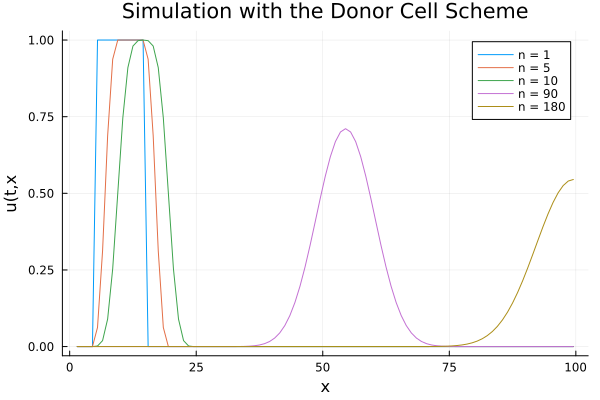
\includegraphics[width=0.66\linewidth]{./images/rectangle-simulation-donorcell.png}
    \caption{Numerical solution of the donor cell scheme for the linear advection equation.}
    \label{fig:sim-donorcell}
\end{figure}

The leapfrog scheme performs the worst compared to the other schemes, as we see large oscillations
at advanced time steps. This leads to a large RMSE and it does not conserve the (positive) mass and
it undershoots frequently. The simulation using the leapfrog can be seen in 
figure~\ref{fig:sim-leapfrog}.

\begin{figure}
    \centering
    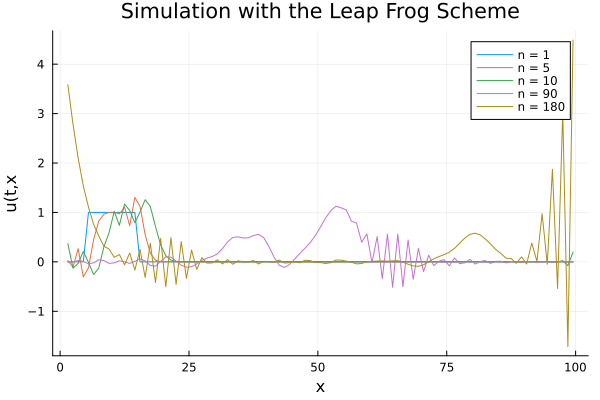
\includegraphics[width=0.66\linewidth]{./images/rectangle-simulation-leapfrog.png}
    \caption{Numerical solution of the leapfrog scheme for the linear advection equation.}
    \label{fig:sim-leapfrog}
\end{figure}

The Runge-Kutta time integrator for the method of lines has a comparable RMSE to other methods;
see figure~\ref{fig:rmse}, but it has worse mass conservation properties as we see in
table~\ref{tab:diag} and figures~\cref{fig:mr,fig:rmp}. We also see oscillations which cause the
mass dissipation, but they have a smaller amplitude than the solution, as it can be seen in
figure~\ref{fig:sim-rk4}.

\begin{figure}
    \centering
    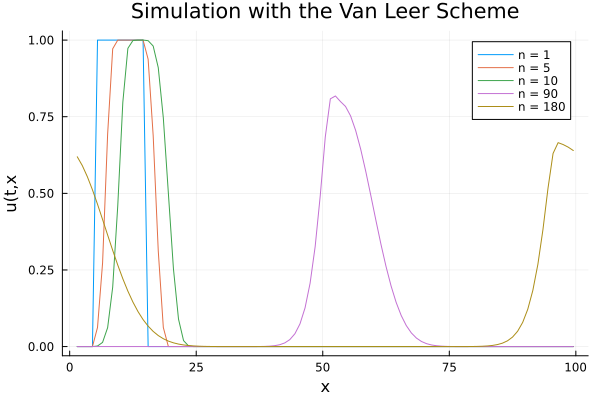
\includegraphics[width=0.66\linewidth]{./images/rectangle-simulation-vanleer.png}
    \caption{Caption}
    \label{fig:}
\end{figure}

The Lax-Wendroff scheme as a finite volume method has good approximation properties as it has a 
RMSE comparable to the other schemes and conserves the mass quite well. However, we can see a small
mass increase but smaller than the leapfrog scheme or the method of lines. We also observe 
over and undershoots, which are often not physical. See also figure~\cref{fig:sim-laxwendroff}.

\begin{figure}
    \centering
    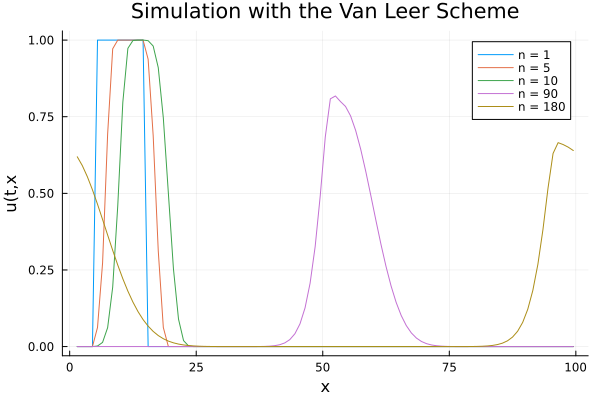
\includegraphics[width=0.66\linewidth]{./images/rectangle-simulation-vanleer.png}
    \caption{Numerical solution of the Lax Wendroff scheme for the linear advection equation.}
    \label{fig:sim-laxwendroff}
\end{figure}

However, the van-Leer scheme shows better mass conservation properties and energy properties; see
\cref{fig:mdr,fig:rm}. Furthermore, it does not exhibit any oscillations but smears at the end of
our simulation. See figure~\cref{fig:sim-vanleer} for the simulation of the van Leer scheme.

\begin{figure}
    \centering
    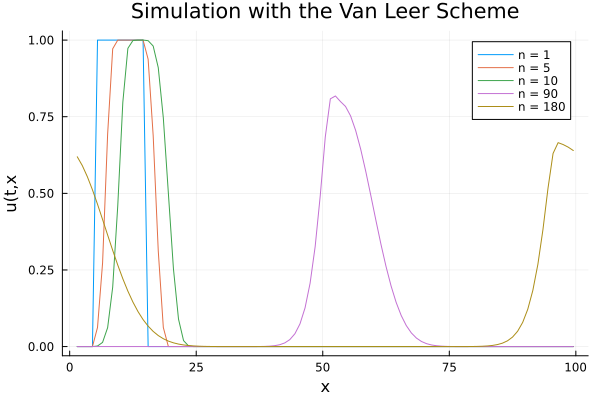
\includegraphics[width=0.66\linewidth]{./images/rectangle-simulation-vanleer.png}
    \caption{Numerical solution of the van Leer scheme for the linear advection equation.}
    \label{fig:sim-vanleer}
\end{figure}


\begin{figure}[h]
    \centering

    % Row 1
    \begin{subfigure}[b]{0.3\textwidth}
        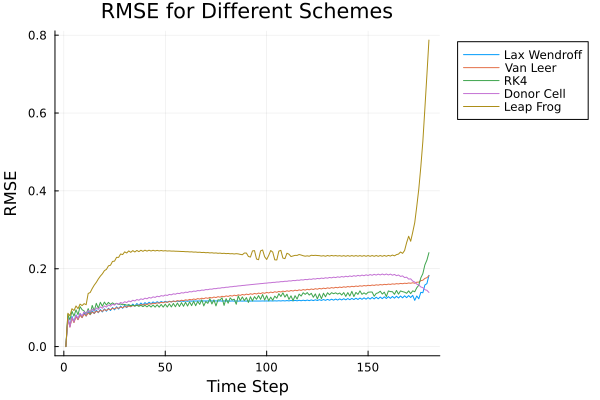
\includegraphics[width=\textwidth]{./images/rectangle-RMSE.png}
        \caption{RMSE for different schemes for the model problem.}
        \label{fig:rmse}
    \end{subfigure}
    \hfill
    \begin{subfigure}[b]{0.3\textwidth}
        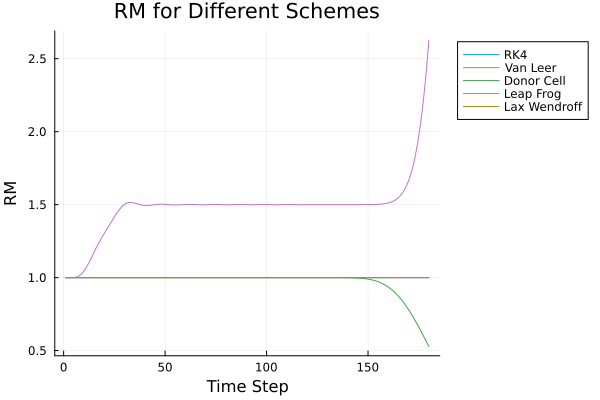
\includegraphics[width=\textwidth]{./images/rectangle-RM.png}
        \caption{Mass ratio $\mathrm{RM}$ for different schemes for the model problem.}
        \label{fig:rm}
    \end{subfigure}
    \hfill
    \begin{subfigure}[b]{0.3\textwidth}
        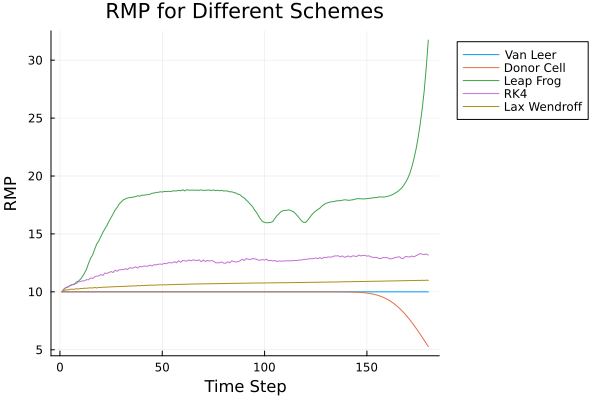
\includegraphics[width=\textwidth]{./images/rectangle-RMP.png}
        \caption{Positive mass ration $\mathrm{RMP}$ for different schemes for the model problem.}
        \label{fig:rm}
    \end{subfigure}

    \vspace{0.5cm} % Space between rows

    % Row 2
    \begin{subfigure}[b]{0.3\textwidth}
        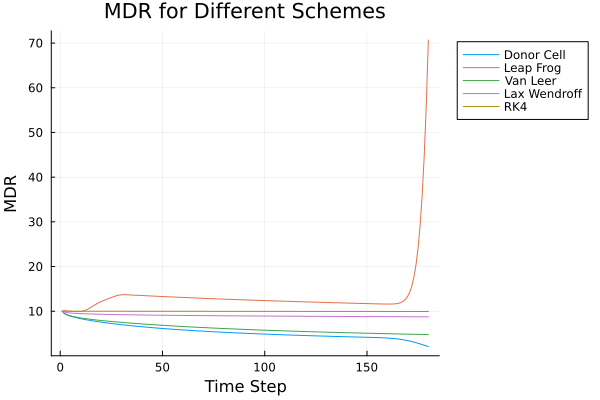
\includegraphics[width=\textwidth]{./images/rectangle-MDR.png}
        \caption{Energy ratio for different schemes for the model problem.}
        \label{fig:mdr}
    \end{subfigure}
    \hfill
    \begin{subfigure}[b]{0.3\textwidth}
        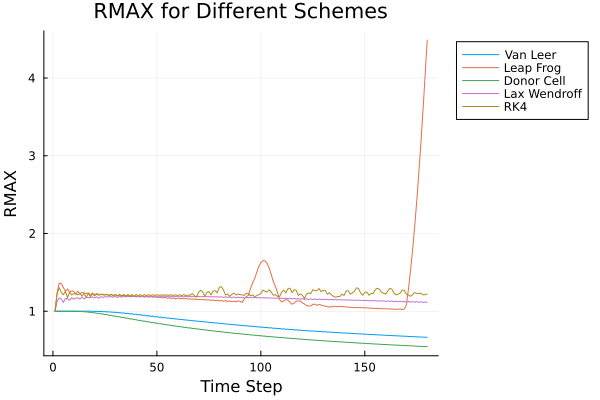
\includegraphics[width=\textwidth]{./images/rectangle-RMAX.png}
        \caption{Maximal amplitude of the numerical solution compared to the initial range.}
        \label{fig:rmax}
    \end{subfigure}
    \hfill
    \begin{subfigure}[b]{0.3\textwidth}
        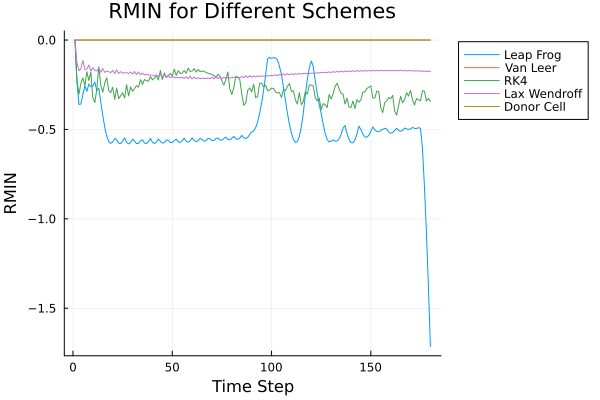
\includegraphics[width=\textwidth]{./images/rectangle-RMIN.png}
        \caption{Minimal amplitude of the numerical solution compared to the initial range.}
        \label{fig:rmix}
    \end{subfigure}

    \caption{Diagnostics for the model problem over time.}
    \label{fig:diagnostics}
\end{figure}






\section{Conclusion}

We conclude that each scheme has some advantages and disadvantages, but none of these capture 
the shocks effectively, as some of them lead to oscillations or smear out during time or do not
conserve the mass or lead to non-physical solutions. The leapfrog scheme is standing out negatively, 
due to the high oscillations and its instability. The van-Leer scheme, as the first proposed
total variation diminishing scheme, captures the shock quite well and conserves the mass and energy.

From here on, we can ask several questions for further research:
\begin{enumerate}
    \item Is there a numerical scheme which conserved the total variation of the numerical
    solution on a regular grid? It can be shown that the total variation of the 
    van-Leer scheme is non-increasing, however it decreases. If such a scheme exists, does
    it conserve the mass or other conserved quantities?

    \item A crucial assumption in our implementation is that the cell interfaces have a constant
    size. How can we transfer these methods to more non-regular geometries as these occur
    regularly in the real world, for example modeling meandering rivers or low altitude winds.
\end{enumerate}
